% !TEX program = pdflatex
\documentclass[aspectratio=169, 11pt]{beamer}

\usetheme{default}
\usecolortheme{default}
\setbeamertemplate{navigation symbols}{}
\setbeamertemplate{footline}[frame number]
\setbeamertemplate{frametitle}{\vspace{0.5em}\textbf{\insertframetitle}}

\usepackage{amsmath,amssymb}
\usepackage{graphicx}
\usepackage{booktabs}
\usepackage{colortbl}
\usepackage{xcolor}
\usepackage{pgfpages}

% Speaker notes on right side
\setbeameroption{show notes on second screen=right}

\graphicspath{{../}}

\definecolor{resultbg}{HTML}{E8F5E9}
\definecolor{highlight}{HTML}{1565C0}

\title{Week 2 Update}
\author{Michael Fang}
\date{March 2026}

\begin{document}

%----------------------------------------------------------------------
\begin{frame}
\centering
\vspace{2em}
{\Large\textbf{Week 2 Update}}

\vspace{1em}
Michael Fang

\vspace{0.5em}
March 2026
\end{frame}
\note{
Weekly progress meeting with Professor Torquato.

Main topics:
\begin{itemize}
  \item Recap of last week
  \item New patterns analyzed (Classes II, III)
  \item The Bombieri-Taylor result
  \item Updated ranking
\end{itemize}
}

%----------------------------------------------------------------------
\begin{frame}{Quick Recap: Last Week}

Last week:
\begin{itemize}
    \item Variance code validated (Poisson benchmark, 1.1\% error)
    \item Three metallic-mean chains: Fibonacci, Silver, Bronze
    \item All gave $\alpha = 3$ as expected
\end{itemize}

\vspace{0.5em}
\begin{table}
\centering
\begin{tabular}{lccc}
\toprule
\textbf{Pattern} & $\boldsymbol{\alpha}$ (measured) & $\boldsymbol{\alpha}$ (expected) & $\boldsymbol{\bar{\Lambda}}$ \\
\midrule
Fibonacci & 3.05 & 3 & 0.200 \\
Silver & 2.99 & 3 & 0.250 \\
Bronze & 2.99 & 3 & 0.282 \\
\bottomrule
\end{tabular}
\end{table}

\vspace{0.5em}
\textbf{This week:} Cover all three hyperuniformity classes and find something in the $1 < \alpha < 2$ gap.
\end{frame}
\note{
Quick reminder of where we left off.

The metallic means all give $\alpha = 3$ because of the 2x2 matrix constraint: $|\lambda_2| = 1/|\lambda_1|$.

Goal this week was to expand beyond just $\alpha = 3$.
}

%----------------------------------------------------------------------
\begin{frame}{Class II: Period-Doubling}

The Period-Doubling chain:
\[
S \to L, \quad L \to LSS \qquad \Rightarrow \qquad M = \begin{pmatrix} 0 & 2 \\ 1 & 1 \end{pmatrix}
\]

\vspace{0.5em}
Matrix gives $\lambda_1 = 2$, $|\lambda_2| = 1$

\vspace{0.3em}
So: $\displaystyle\alpha = 1 - \frac{2\ln(1)}{\ln(2)} = 1$

\vspace{0.5em}
\textbf{Results:}
\begin{itemize}
    \item Variance grows like $\ln R$ (not bounded, not power-law)
    \item $\bar{\Lambda}$ diverges --- can't use it to rank this pattern
    \item This is the boundary case: $\alpha = 1$ exactly
    \item \colorbox{resultbg}{Class II confirmed}
\end{itemize}
\end{frame}
\note{
Period-Doubling is the boundary case: $\alpha = 1$ exactly.

$|\lambda_2| = 1$ means $\ln(1) = 0$ in the formula.

First Class II example --- variance grows logarithmically.
}

%----------------------------------------------------------------------
\begin{frame}{Class III: 0222 Chain}

The 0222 chain:
\[
S \to LL, \quad L \to SSLL
\]

\begin{columns}[T]
\begin{column}{0.45\textwidth}
\vspace{0.5em}
Here $|\lambda_2| = \sqrt{5} - 1 > 1$

So: $\alpha \approx 0.64$

\vspace{0.5em}
\textbf{Results:}
\begin{itemize}
    \item Variance grows like $R^{0.36}$
    \item $\bar{\Lambda}$ diverges
    \item Class III confirmed
\end{itemize}

\vspace{0.5em}
Now have examples of all three classes.
\end{column}

\begin{column}{0.55\textwidth}
\centering
\small
\textbf{The three classes:}
\vspace{0.3em}

\begin{tabular}{lcc}
\toprule
\textbf{Class} & $\boldsymbol{\alpha}$ & $\boldsymbol{\sigma^2(R)}$ \\
\midrule
I & $> 1$ & bounded \\
II & $= 1$ & $\sim \ln R$ \\
III & $< 1$ & $\sim R^{1-\alpha}$ \\
\bottomrule
\end{tabular}

\vspace{1em}
The exponent $1 - 0.64 = 0.36$ matches the measured value.
\end{column}
\end{columns}
\end{frame}
\note{
0222 has $|\lambda_2| > 1$, which gives $\alpha < 1$.

The power-law growth $R^{0.36}$ matches the prediction $R^{1-\alpha}$.

All three classes now covered.
}

%----------------------------------------------------------------------
\begin{frame}{URL Verification}

Tested the perturbed lattice formula (Klatt et al.\ 2020):
\[
\bar{\Lambda}(a) = \frac{1+a^2}{6}
\]

\begin{columns}[T]
\begin{column}{0.45\textwidth}
\vspace{0.5em}
\textbf{Numerical results:}
\begin{center}
\begin{tabular}{ccc}
\toprule
$a$ & Numerical & Exact \\
\midrule
0.1 & 0.168 & 0.168 \\
0.5 & 0.208 & 0.208 \\
1.0 & 0.334 & 0.333 \\
\bottomrule
\end{tabular}
\end{center}

\vspace{0.3em}
Errors $< 0.3\%$ --- validates the code against an independent analytical result.
\end{column}

\begin{column}{0.55\textwidth}
\centering
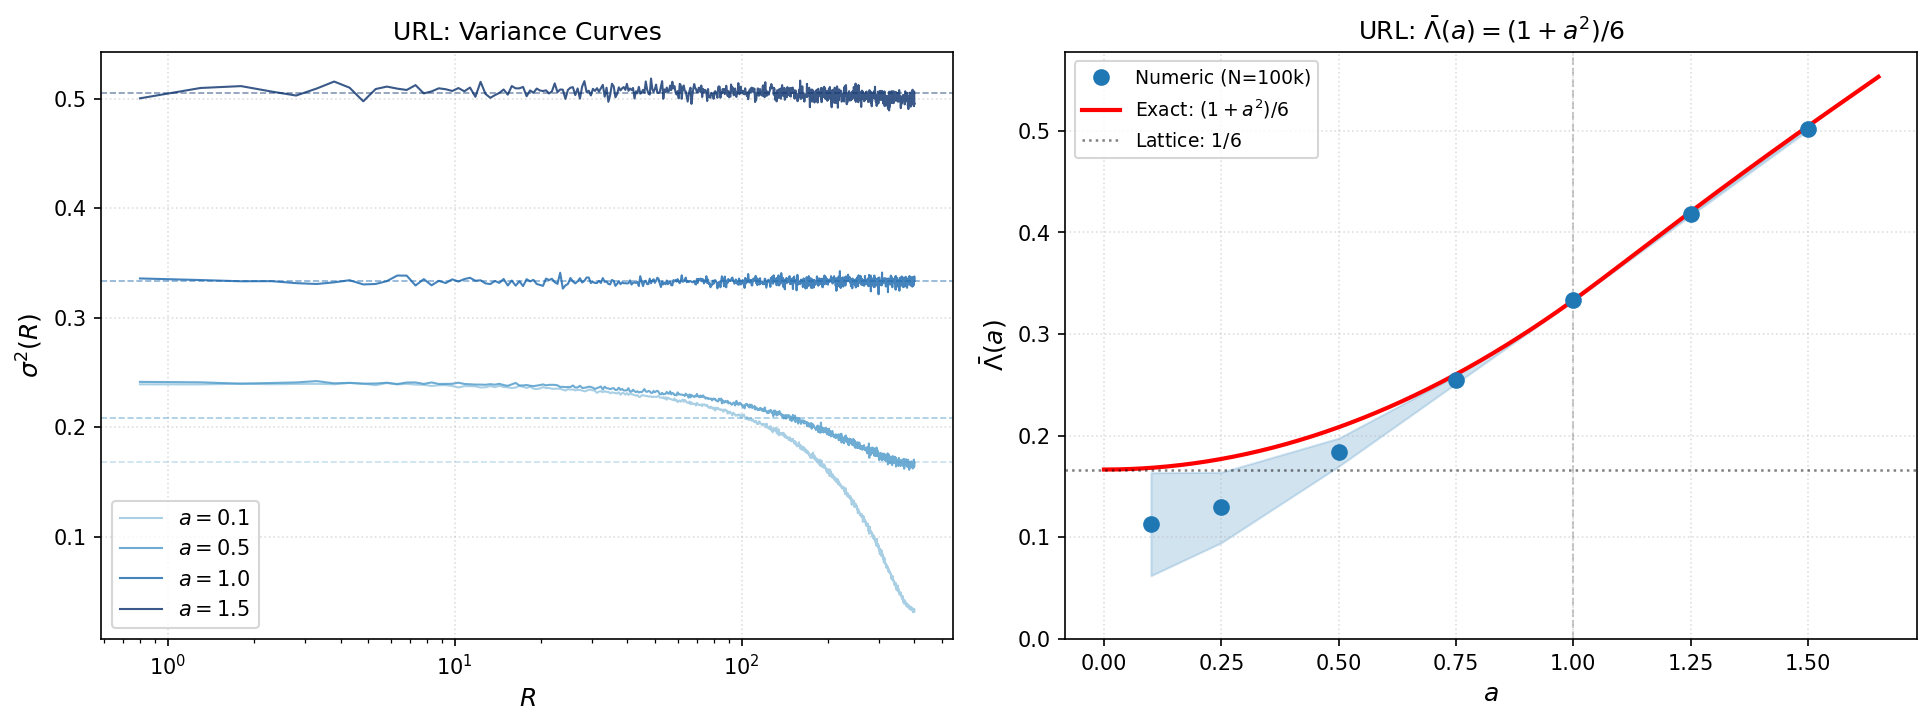
\includegraphics[width=\linewidth]{figures/figB_url_analysis.png}
\end{column}
\end{columns}
\end{frame}
\note{
URL = uncorrelated random lattice (independent displacements on integer lattice).

Exact formula from Klatt et al.\ (2020): $\bar{\Lambda}(a) = (1+a^2)/6$.
Recovers lattice value $1/6$ at $a=0$; equals $1/3$ at $a=1$ (cloaking threshold).

Good independent validation because we have an analytical result for all $a$.
Always $\alpha = 2$ regardless of displacement amplitude $a$.
}

%----------------------------------------------------------------------
\begin{frame}{Stealthy Patterns}

Analyzed stealthy configurations provided by Sam.

\vspace{0.2em}
\textbf{Idea:} Force $S(k) = 0$ for all $|k| < K^*$, not just at $k = 0$.

\vspace{0.3em}
\begin{columns}[T]
\begin{column}{0.45\textwidth}
\textbf{Results} ($N = 2{,}000$, $\sim$4000 configs each):
\vspace{0.2em}
\begin{center}
\small
\begin{tabular}{cccc}
\toprule
$\chi$ & $\bar{\Lambda}$ & $\bar{\Lambda}_\text{pred}$ & $\alpha$ \\
\midrule
0.1 & 1.02 & 1.01 & 2.0 \\
0.2 & 0.53 & 0.51 & 2.0 \\
0.3 & 0.36 & 0.34 & 2.0 \\
\bottomrule
\end{tabular}
\end{center}

\vspace{0.4em}
$\bar{\Lambda} \approx 1/(\pi^2 \chi)$ --- matches theory.

\vspace{0.3em}
Higher $\chi$ $\Rightarrow$ wider exclusion zone $\Rightarrow$ better suppression.
\end{column}

\begin{column}{0.55\textwidth}
\centering
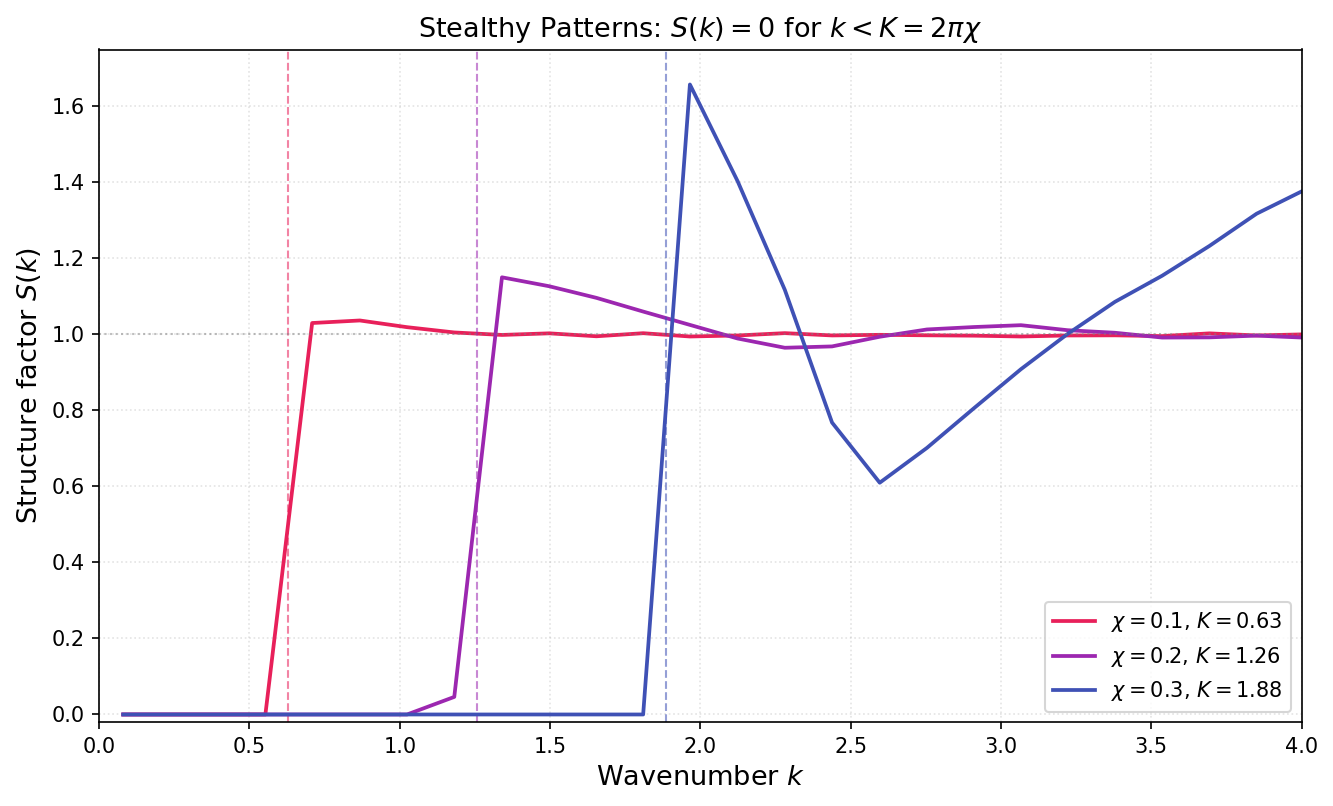
\includegraphics[width=\linewidth]{figures/stealthy_Sk_overlay.png}

\vspace{0.1em}
{\footnotesize $S(k)$ averaged over all configs for each $\chi$. Shaded region = exclusion zone.}
\end{column}
\end{columns}
\end{frame}
\note{
Data from another grad student (CCO format, ~4000 configs per $\chi$).

$\chi$ controls the size of the exclusion region: $K = 2\pi\chi$.

Theory predicts $\bar{\Lambda} \approx 1/(\pi^2 \chi)$.

The overlay shows all three $\chi$ values on one plot --- the exclusion zone widens visibly as $\chi$ increases, and $S(k)$ rises sharply at $K^*$ before approaching 1 at large $k$.

$\alpha = 2$ is theoretical (can't extract via spreadability due to exponential decay).
}

%----------------------------------------------------------------------
\begin{frame}{Filling the $1 < \alpha < 2$ Gap}

There was a gap in the $\alpha$ coverage:

\vspace{0.3em}
\begin{center}
\begin{tabular}{lcl}
\toprule
$\alpha$ & Class & Examples \\
\midrule
3 & I & Fibonacci, Silver, Bronze \\
2 & I & URL, Stealthy \\
\rowcolor{yellow!30}
$1 < \alpha < 2$ & I & No quasicrystal \\
1 & II & Period-Doubling \\
$< 1$ & III & 0222 \\
\bottomrule
\end{tabular}
\end{center}

\vspace{0.5em}
The issue: all 2$\times$2 metallic-mean matrices give $\alpha = 3$ because $|\lambda_2| = 1/|\lambda_1|$.

\vspace{0.3em}
Solution: the Bombieri-Taylor cubic substitution (1986 paper, p. C3-21).
\end{frame}
\note{
The 2x2 constraint: det$(M) = \pm 1$ forces $|\lambda_2| = 1/|\lambda_1|$.

This always gives $\alpha = 1 + 2 = 3$.

Need a 3x3 matrix to break this constraint.
}

%----------------------------------------------------------------------
\begin{frame}{Bombieri-Taylor Cubic Substitution}

From the 1986 paper (p. C3-21):

\begin{columns}[T]
\begin{column}{0.45\textwidth}
\vspace{0.3em}
\textbf{Three-letter alphabet:}
\[
a \to aac, \; b \to ac, \; c \to b
\]

\textbf{Matrix:}
\[
M = \begin{pmatrix} 2 & 0 & 1 \\ 1 & 0 & 1 \\ 0 & 1 & 0 \end{pmatrix}
\]

Eigenvalues: $\theta_1 = 2.247$, $|\lambda_2| = 0.802$
\end{column}

\begin{column}{0.55\textwidth}
\textbf{Predicted:}
\[
\alpha = 1 - \frac{2\ln(0.802)}{\ln(2.247)} = \colorbox{resultbg}{\textbf{1.545}}
\]

\vspace{0.5em}
\textbf{Implementation:}
\begin{itemize}
    \item Extended code for 3-letter alphabets
    \item Generated 9.5 million points
    \item Computed variance and $\bar{\Lambda}$
\end{itemize}

\vspace{0.5em}
\textbf{Result:} $\bar{\Lambda} = 0.377$, Class I confirmed.
\end{column}
\end{columns}
\end{frame}
\note{
Key: $|\lambda_2| = 0.802 \neq 1/\theta_1 = 0.445$.

The 3x3 matrix breaks the constraint.

$\theta_1$ is a Pisot number (conjugates all $< 1$).
}

%----------------------------------------------------------------------
\begin{frame}{Bombieri-Taylor Results}
\centering
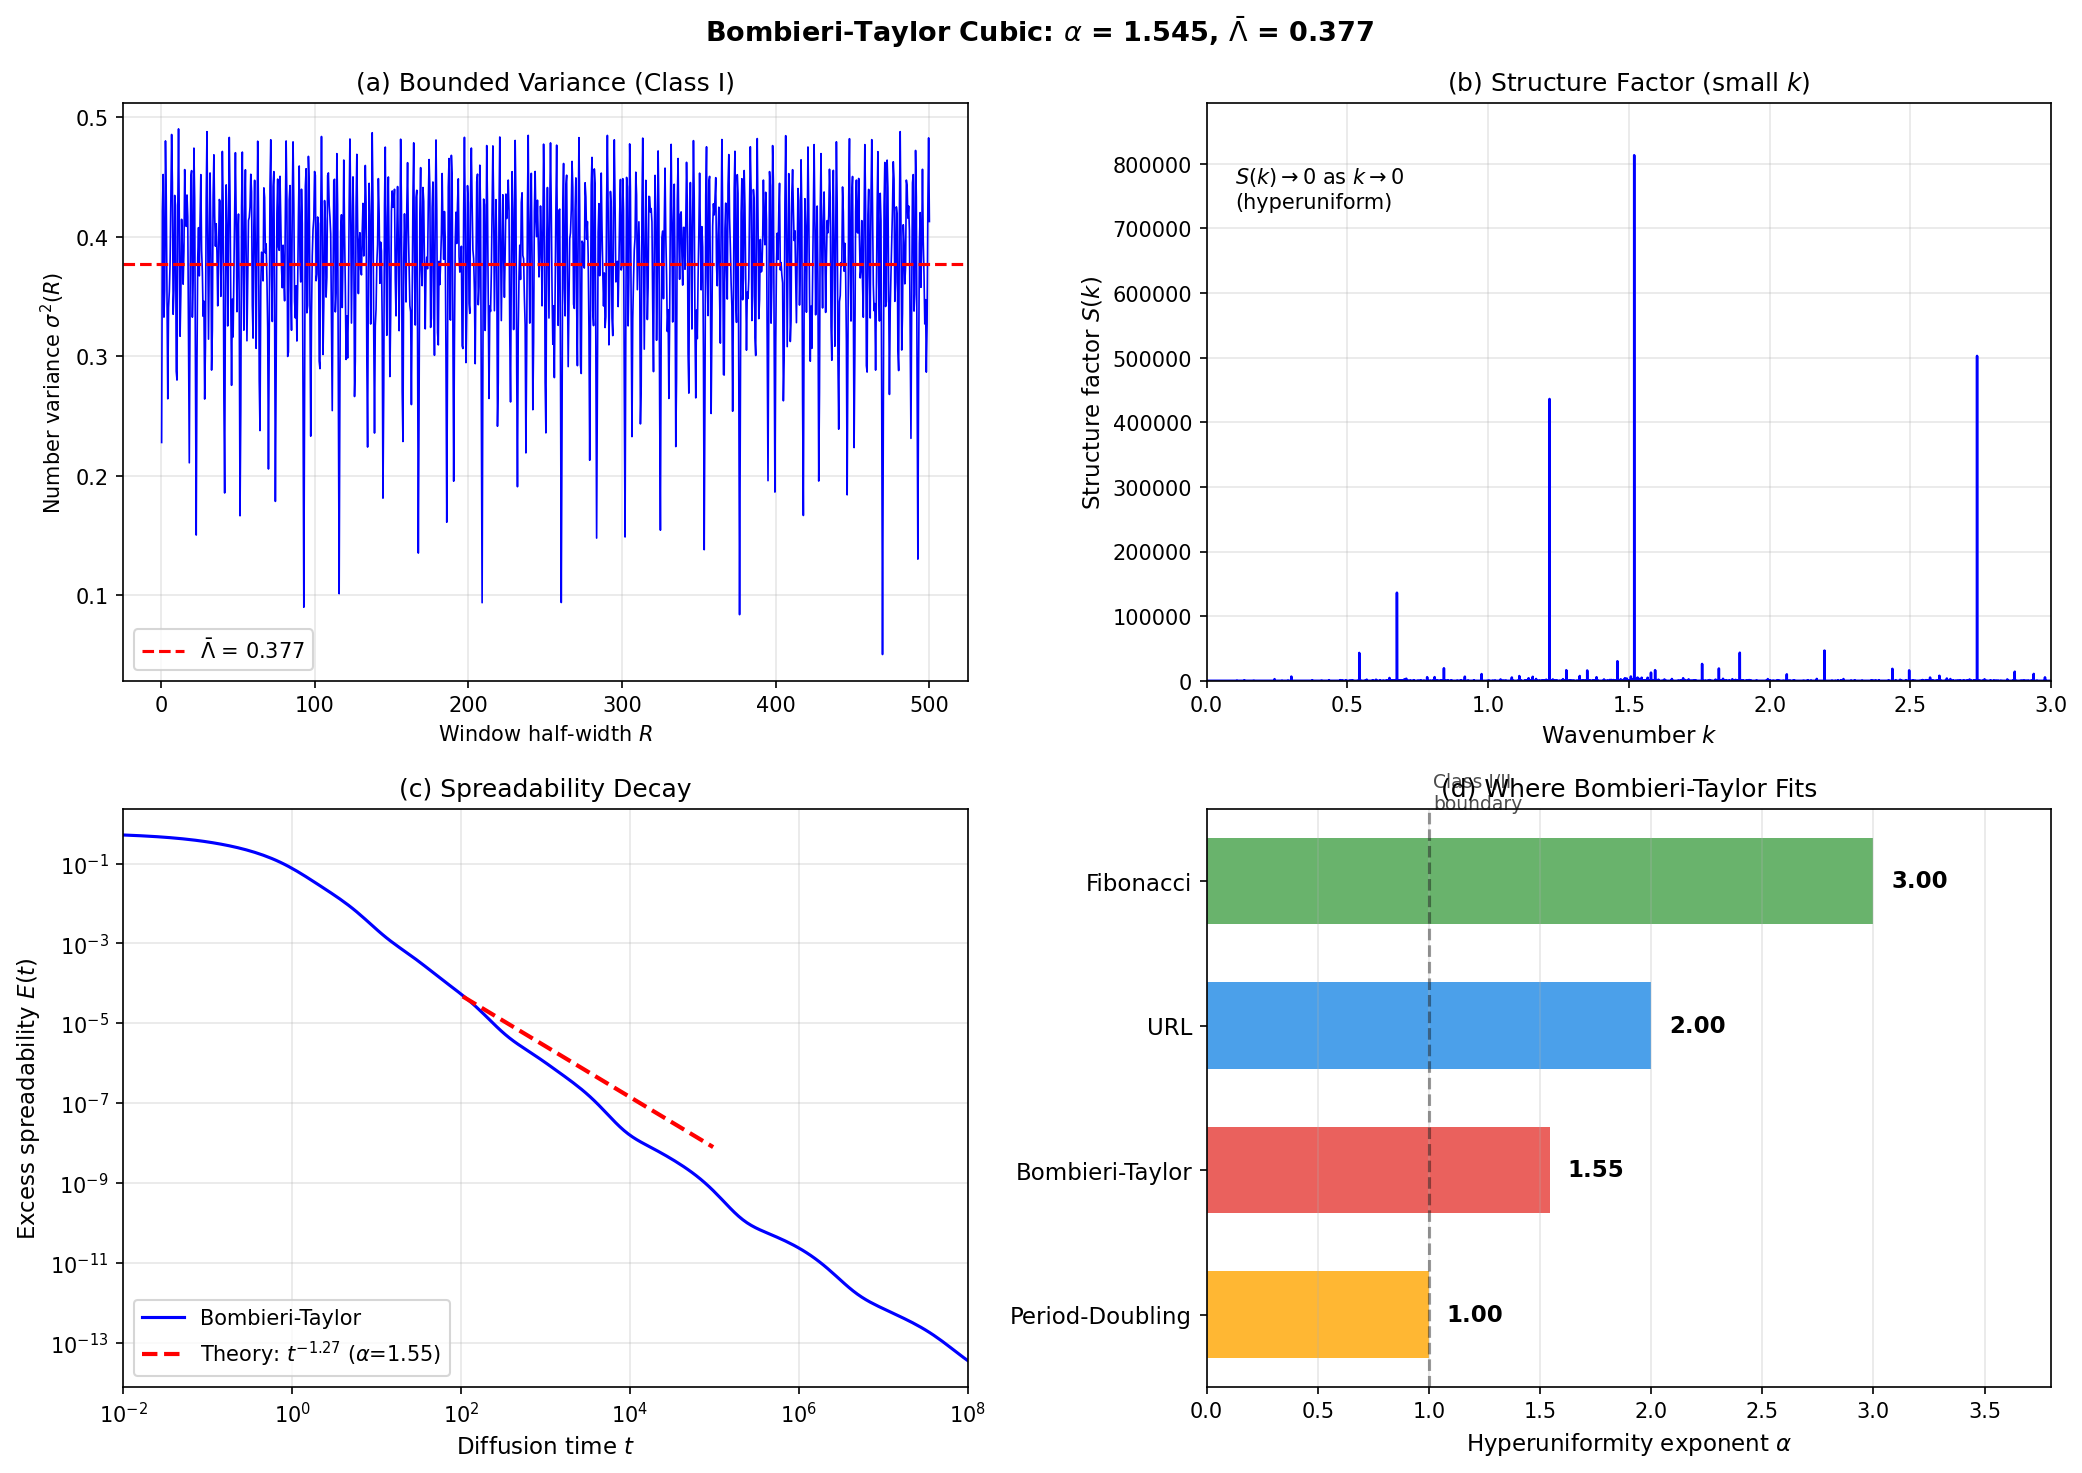
\includegraphics[width=0.66\linewidth]{figures/bombieri_taylor_analysis.png}

\vspace{0.1em}
\small
Variance is bounded (Class I). Log-periodic oscillations in spreadability are expected for quasicrystals.
\end{frame}
\note{
\textbf{Panel (a)}: Bounded variance confirms Class I. Oscillates between 0.05--0.49, mean = 0.377.

\textbf{Panel (b)}: Structure factor at small $k$. Shows $S(k) \to 0$ as $k \to 0$ (hyperuniform). Bragg peaks are characteristic of quasicrystals.

\textbf{Panel (c)}: Spreadability decay. The log-periodic oscillations make power-law fitting unreliable for quasicrystals. The eigenvalue formula is exact; spreadability fit is not.

\textbf{Panel (d)}: Shows Bombieri-Taylor fills the gap between Period-Doubling ($\alpha=1$) and URL ($\alpha=2$).

\textbf{Confidence}: $\alpha = 1.545$ is exact (analytical from eigenvalues). $\bar{\Lambda} = 0.377$ is numerical average of bounded variance.
}

%----------------------------------------------------------------------
\begin{frame}{Updated Ranking}

Here's where everything stands now:

\vspace{0.3em}
\small
\centering
\begin{tabular}{lccc}
\toprule
\textbf{Pattern} & \textbf{Class} & $\boldsymbol{\alpha}$ & $\boldsymbol{\bar{\Lambda}}$ \\
\midrule
Lattice               & I & $\infty$ & 0.167 \\
URL ($a=0.1$)         & I & 2.0      & 0.168 \\
Fibonacci             & I & 3.0      & 0.200 \\
Silver                & I & 3.0      & 0.250 \\
Bronze                & I & 3.0      & 0.282 \\
Copper                & I & 3.0      & 0.293 \\
Nickel                & I & 3.0      & 0.310 \\
URL ($a=1.0$)         & I & 2.0      & 0.333 \\
Stealthy ($\chi=0.3$) & I & 2.0      & 0.358 \\
\rowcolor{resultbg}
\textbf{Bombieri-Taylor} & \textbf{I} & \textbf{1.545} & \textbf{0.377} \\
\midrule
Period-Doubling       & II  & 1.0  & diverges \\
0222                  & III & 0.64 & diverges \\
\bottomrule
\end{tabular}
\end{frame}
\note{
26 patterns total (counting all URL/Gaussian/Stable/Stealthy variants).
Table shows a selected subset sorted by $\bar{\Lambda}$ within each class.

Copper ($\bar{\Lambda}=0.293$) and Nickel ($\bar{\Lambda}=0.310$) fill the gap between
Bronze (0.282) and URL $a=1.0$ (0.333) in the metallic-mean family.

Bombieri-Taylor fills the gap between $\alpha = 1$ and $\alpha = 2$.

First quasicrystal with $1 < \alpha < 2$.
}

%----------------------------------------------------------------------
\begin{frame}{Summary}

\textbf{This week:}
\begin{itemize}
    \item Added Class II (Period-Doubling, $\alpha = 1$)
    \item Added Class III (0222, $\alpha = 0.64$)
    \item Verified URL formula to $< 0.3\%$
    \item Analyzed stealthy data ($\bar{\Lambda} \approx 1/(\pi^2\chi)$)
    \item Implemented Bombieri-Taylor cubic ($\alpha = 1.545$)
\end{itemize}

\vspace{0.5em}
\textbf{Main result:} Filled the $1 < \alpha < 2$ gap with a quasicrystal.

\vspace{0.5em}
\textbf{Questions:}
\begin{itemize}
    \item Are there other cubic/quartic substitutions to try?
    \item Should 2D generalizations be next?
\end{itemize}
\end{frame}
\note{
Total patterns analyzed: 26

Key accomplishment: Bombieri-Taylor fills the gap.

Possible next steps: other cubic substitutions, 2D/3D.
}

%----------------------------------------------------------------------
\begin{frame}{References}

\small
\begin{itemize}
    \item Torquato \& Stillinger (2003), Phys. Rev. E 68, 041113
    \item Bombieri \& Taylor (1986), J. Physique Colloques 47, C3-19
    \item O\u{g}uz et al. (2017), Phys. Rev. B 95, 054119
    \item Torquato (2021), Phys. Rev. E 104, 054102
\end{itemize}
\end{frame}
\note{
Main references used this week.
}

\end{document}
